\chapter{Motion-Aware Unitを用いた3波長を入力とした紫外線像の全球時系列予測}
  \section{実験概要}
    ここでは、171Å、193Åフィルターで得られたデータを追加で利用し、3波長の入力データから211Åの波長データに対する予測を行った。
    これらの波長は、太陽のコロナ領域における異なる温度帯を観測するためのものであり、予測モデルに多様な物理的情報を提供することが期待される。
    171Åの波長は、太陽のコロナにおける温度が約60万Kの領域を捉えるのに特化しており、193Åの波長は約100万Kの領域を捉える。
    これらの波長から得られる情報を組み合わせることにより、単一の波長では捉えられない層間の相互作用を捉え、より高い精度での予測を可能にすることを期待する。
    
    モデルには先の実験と同じく、MAUを用いる。入力は3波長、すなわち画像的には3チャンネルである。
    目的となる出力は211Åの波長のみであるが、MAUは3チャンネルを出力する。
    これは、「出力シークエンスのタイムステップ1以降では、直前のモデルの出力を入力データとして扱う」という動画予測モデルの一般的な性質によるものである。
    このような性質から、211Åの波長のみを出力として扱うために、出力された3チャンネルのうち、211Åの波長のみを抽出するという処理を行った。
    図\ref{fig:exp2_concept}に本実験の概念図を示す。
    \begin{figure}[htbp]
      \centering
      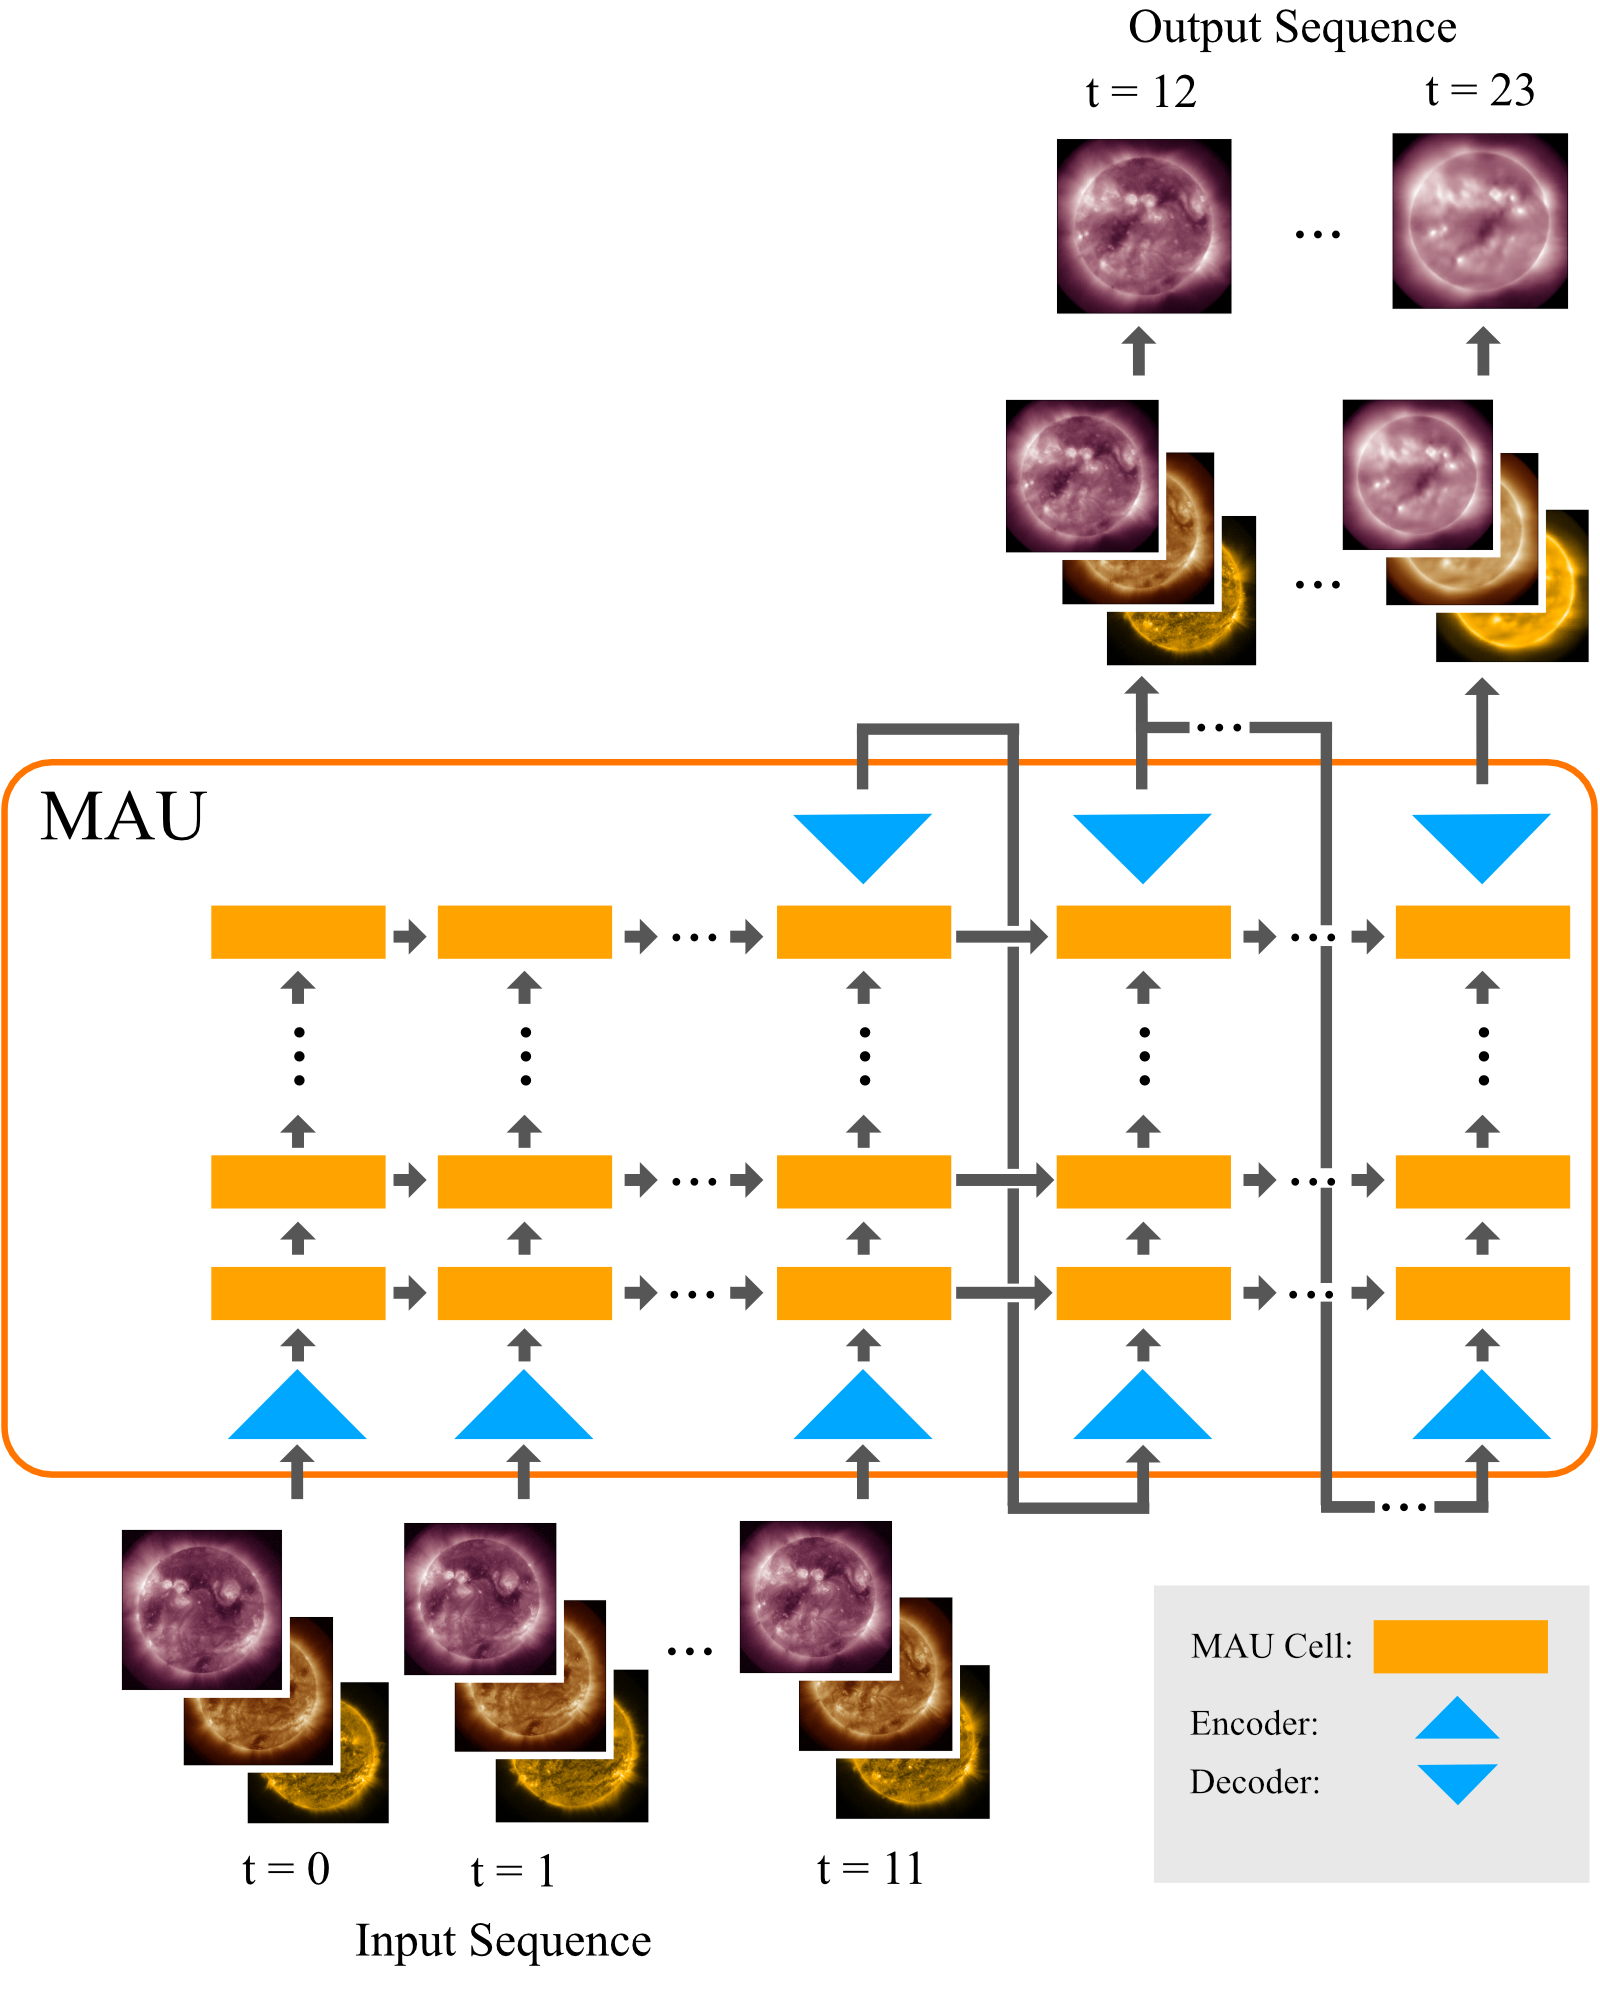
\includegraphics[width=\textwidth]{figures/exp2/exp2_concept.jpg}
      \caption{本実験の概念図。3波長の観測画像を入力として、211Åの波長の観測画像を予測する。}
      \label{fig:exp2_concept}
    \end{figure}

%%%%%%%%%%%%%%%%%%%%%%%%%%%%%%%%%%%%%%%%%%%%%%%%%%%%%%%%%%%%%%%%%%%%%%%%%%%%%%%%%%%%%%%%%%%%%%%%%%%%%%%%%%%%%%%%%%%%%%%%%%%%
%%%%%%%%%%%%%%%%%%%%%%%%%%%%%%%%%%%%%%%%%%%%%%%%%%%%%%%%%%%%%%%%%%%%%%%%%%%%%%%%%%%%%%%%%%%%%%%%%%%%%%%%%%%%%%%%%%%%%%%%%%%%

  \section{実験設定}
    各ハイパーパラメータの設定を表\ref{tab:exp2_hyperparameters}に示す。チャンネル数は入力波長に合わせて3である。
    バッチサイズは2に変更している。これは、NVIDIA RTX A6000のメモリ容量の制約によるものである。
    前回実験と同様に、 学習時間の短縮およびメモリ使用量の削減のため、AMP(\cite{micikevicius2017mixed})を適用した。
    \begin{table}[htbp]
      \centering
      \begin{tabular}{lc}
      \hline
      ハイパーパラメータ & 値 \\
      \hline\hline
      バッチサイズ & 3 \\
      \hline
      エポック数 & 100 \\
      \hline
      学習率 & 0.0005 \\
      \hline
      損失関数 & MSE \\
      \hline
      チャンネル & 3 \\
      \hline
      カーネルサイズ & (5, 5) \\
      \hline
      MAU Cell数 & 16 \\
      \hline
      \end{tabular}
      \caption{本実験でのハイパーパラメータ設定。基本的には前実験と同様であるが、チャンネル数が1から3に変更されている。}
      \label{tab:exp2_hyperparameters}
    \end{table}
    データに関しても、データ数の増減による影響がないように、前回の実験と同じ期間のデータを用いた。欠損期間なども同様である。

%%%%%%%%%%%%%%%%%%%%%%%%%%%%%%%%%%%%%%%%%%%%%%%%%%%%%%%%%%%%%%%%%%%%%%%%%%%%%%%%%%%%%%%%%%%%%%%%%%%%%%%%%%%%%%%%%%%%%%%%%%%%
%%%%%%%%%%%%%%%%%%%%%%%%%%%%%%%%%%%%%%%%%%%%%%%%%%%%%%%%%%%%%%%%%%%%%%%%%%%%%%%%%%%%%%%%%%%%%%%%%%%%%%%%%%%%%%%%%%%%%%%%%%%%

  \section{学習の推移}
    学習の完了までに約40時間を要した。
    損失は図\ref{fig:exp2_learn_progress}のように推移した。
    学習損失、検証損失ともに、安定的に減少していることがわかる。
    前半エポックでは急激な増減が見られるが、後半エポックでは安定的に減少している。
    最終的な値は前回実験よりも高い値を示しているが、これは目的とする211\AA 以外の波長の情報を含んでいるため前回実験との単純な比較はできない。
    \begin{figure}[htbp]
      \centering
      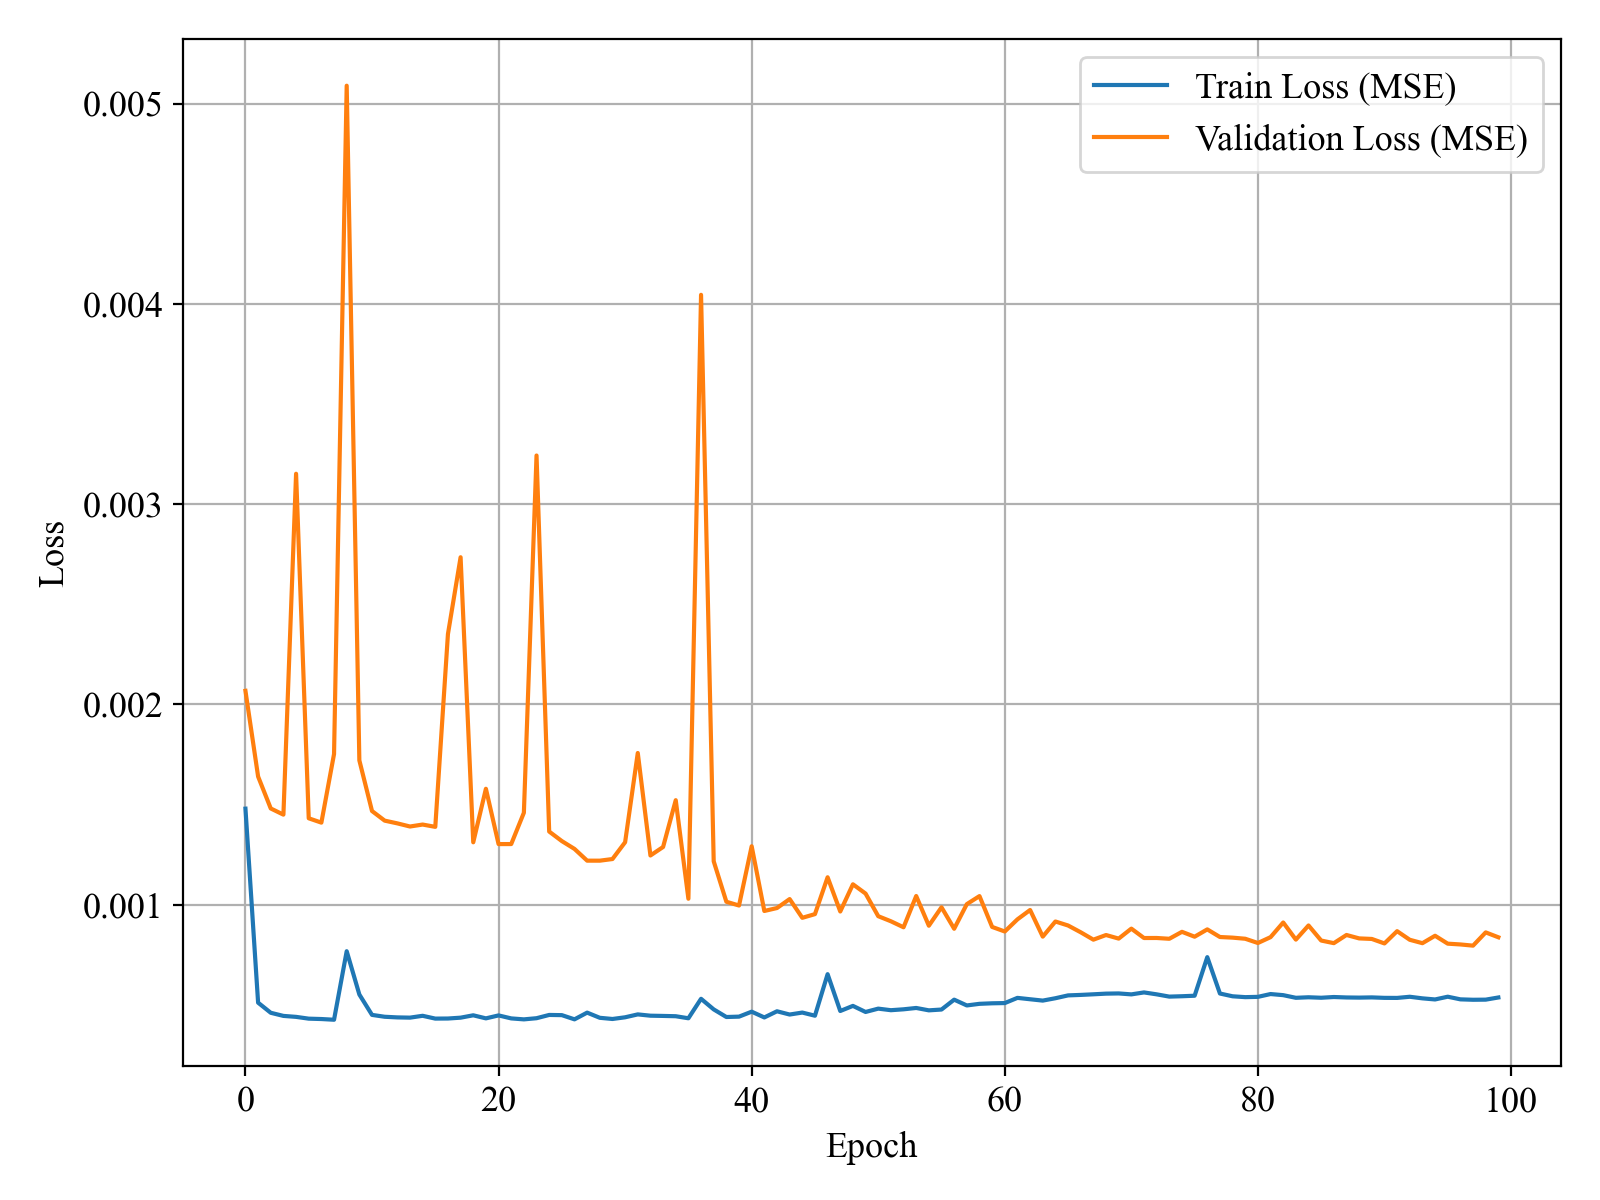
\includegraphics[width=0.8\textwidth]{figures/exp2/loss.png}
      \caption{本実験での、学習データ(青線)、検証データ(オレンジ線)での損失関数の推移。}
      \label{fig:exp2_learn_progress}
    \end{figure}

%%%%%%%%%%%%%%%%%%%%%%%%%%%%%%%%%%%%%%%%%%%%%%%%%%%%%%%%%%%%%%%%%%%%%%%%%%%%%%%%%%%%%%%%%%%%%%%%%%%%%%%%%%%%%%%%%%%%%%%%%%%%
%%%%%%%%%%%%%%%%%%%%%%%%%%%%%%%%%%%%%%%%%%%%%%%%%%%%%%%%%%%%%%%%%%%%%%%%%%%%%%%%%%%%%%%%%%%%%%%%%%%%%%%%%%%%%%%%%%%%%%%%%%%%

  \section{実験結果}
    図\ref{fig:exp2_gt}および図\ref{fig:exp2_pd}に、この実験での出力例を示す。
    予測の生成は、データセット1単位、12枚の生成あたり、約5秒であった。
    \begin{figure}[htbp]
      \centering
      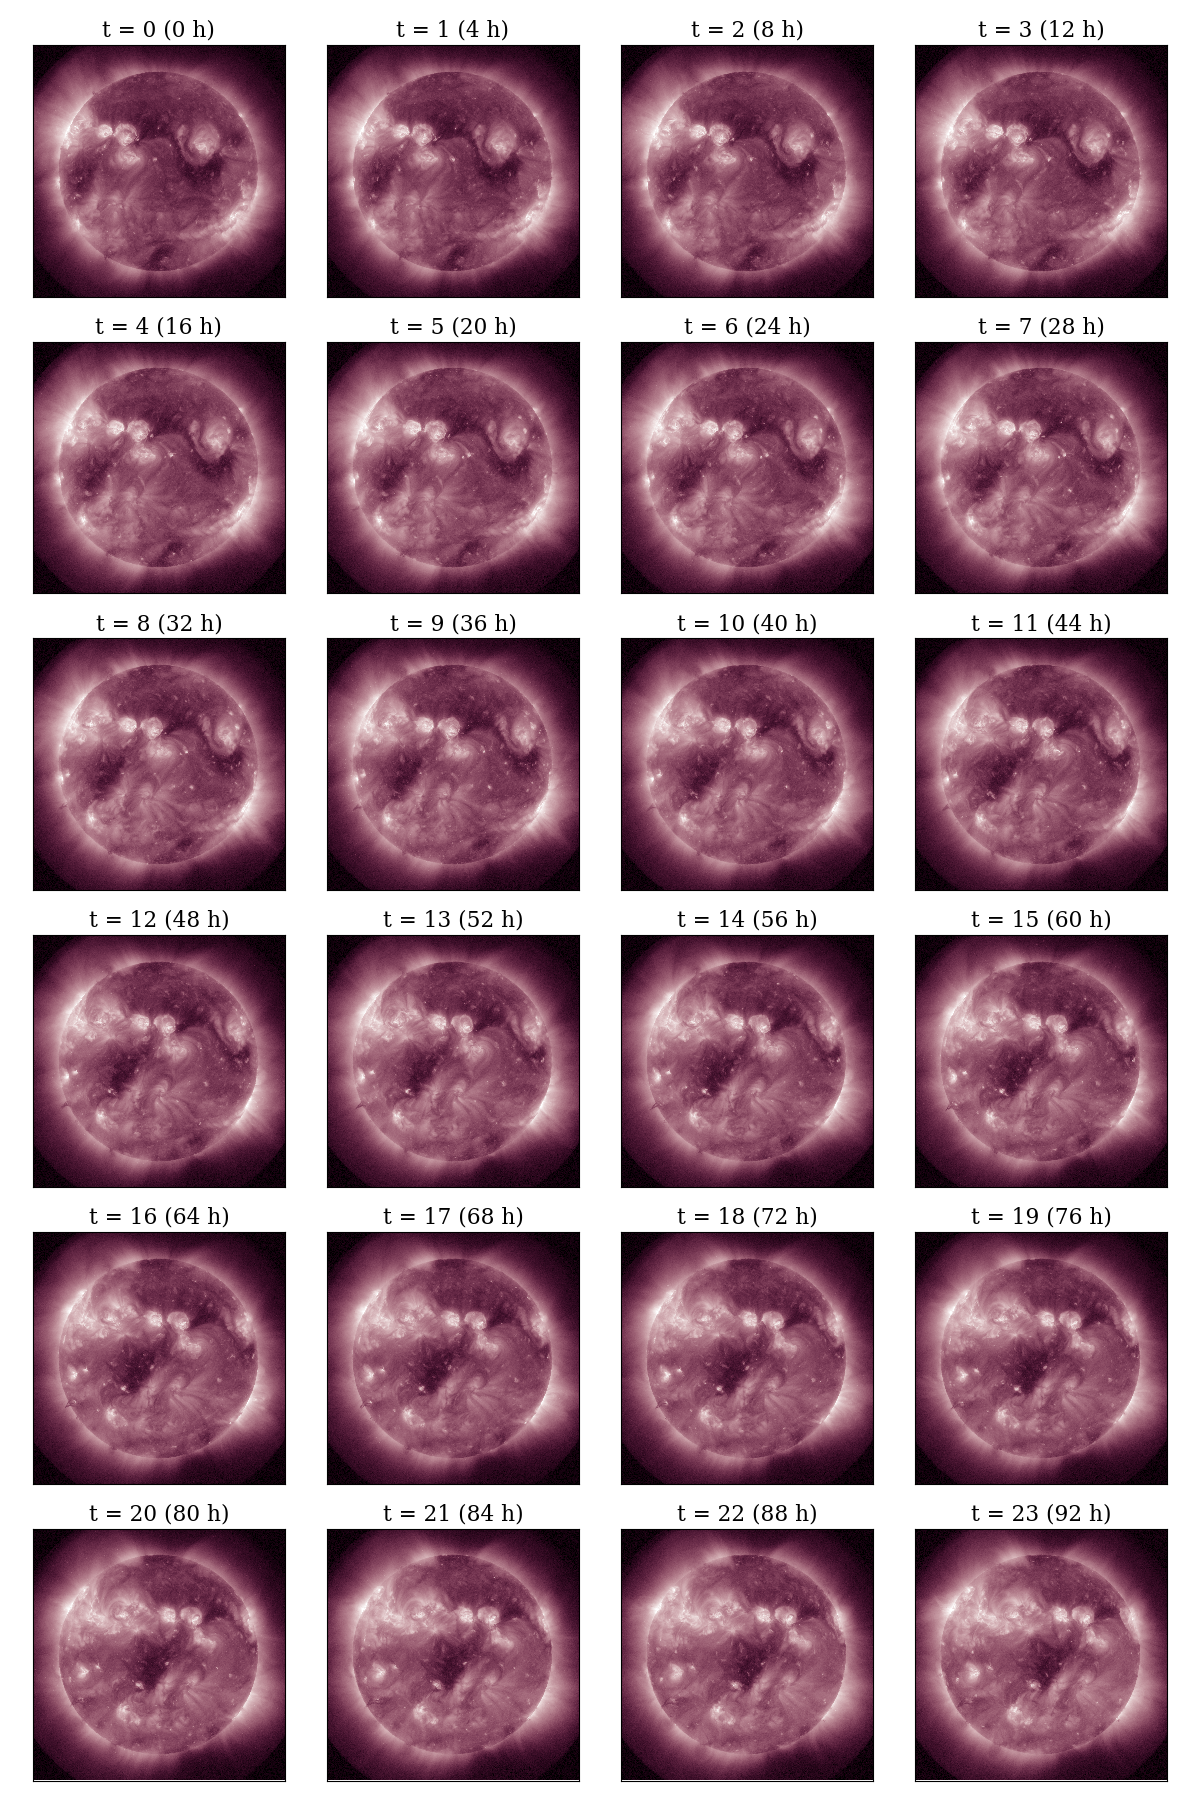
\includegraphics[width=0.95\textwidth]{figures/exp2/gt.png}
      \caption{実際の観測画像の例。2022年2月18日0時から2022年2月22日20時の期間から4時間毎にサンプリングされている。このt=0からt=11までをモデルに入力データとして渡している。モデルはその入力データを元に、t=12からt=23の12枚の画像を予測する。t=12以降の実際の観測画像はモデルに渡されない。}
      \label{fig:exp2_gt}
    \end{figure}
    \begin{figure}[htbp]
      \centering
      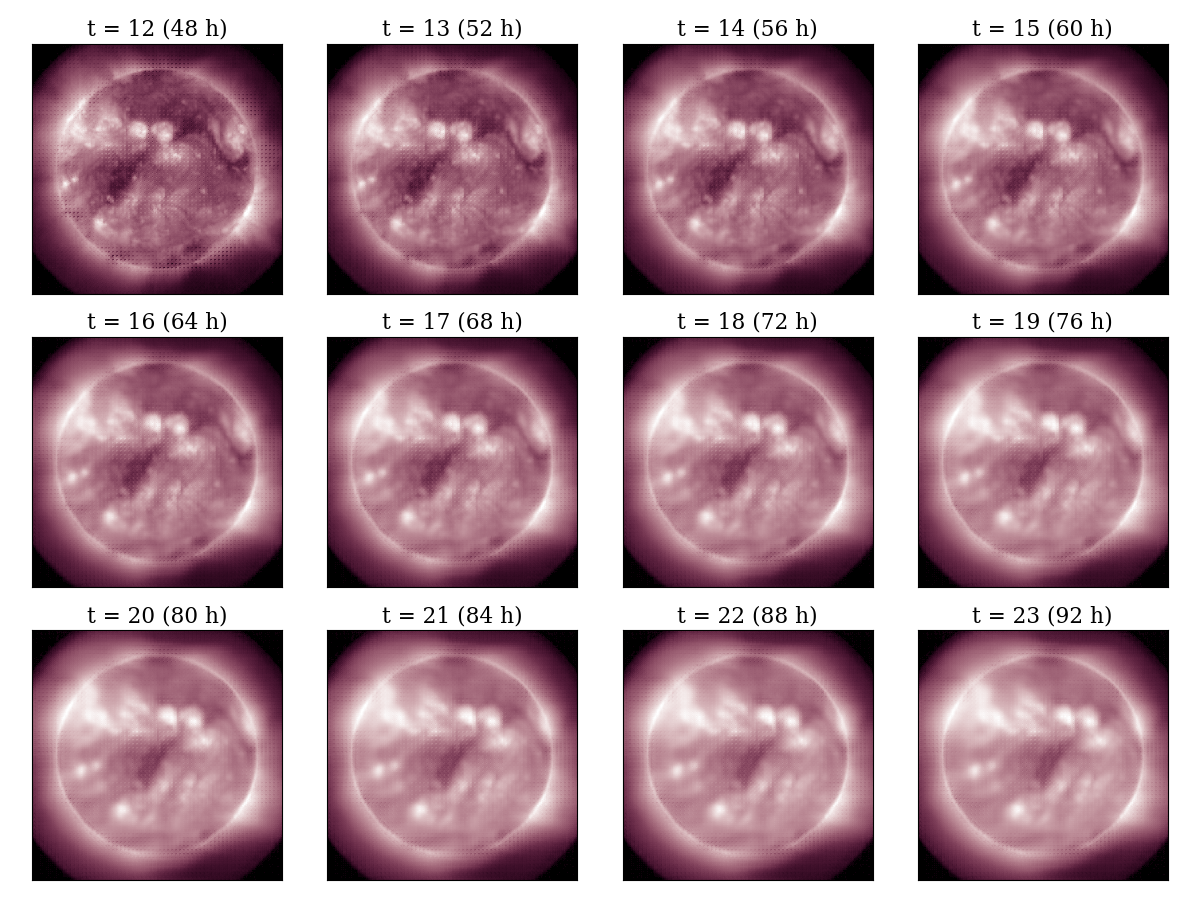
\includegraphics[width=0.95\textwidth]{figures/exp2/pd.png}
      \caption{MAUによる予測画像。対応するタイムステップtの観測画像(図\ref{fig:exp2_gt})と比較することでモデルの再現度を視覚的に評価することができる。大規模な構造は概ね実際の観測画像と合致している。モデルの特性により、時間経過とともに少しずつ予測が不安定になり、ぼやけた見た目になる。}
      \label{fig:exp2_pd}
    \end{figure}
    モデルの出力は、視覚的には実際の観測画像と概ね合致しているが、前回実験と比較すると、よりぼやけが強く、全体的にシャープさに欠けるように見える。
    この実験における評価では、前回の実験と同様の評価を行った。
  
% *************************************************************************************************************
    \subsection{全球での評価}
      はじめに全球での評価を行った。
      前回実験と同様に、まず輝度強度の平均値と実際の平均値との誤差、SSIMを計算した。さらに単純差動回転モデルとの比較も行った。
      また、これらの値の時間経過に対する変化を観察し、より不確定性の高い将来の予測に対しても動画予測モデルが有効であるかを検証した。

      \subsubsection{平均輝度の再現}
        モデルの出力の全球での平均輝度と、実際の観測画像との絶対誤差の推移を図\ref{fig:exp2_error}に示す。
        これは、50のテストセットに対して、各テストセットに含まれる各画像の全球での平均輝度を計算し、その時間ステップごとの平均値を取ったものである。
        また、前回実験と同様に、モデルの予測性能をさらに詳細に評価するために、シンプルな差動回転モデルとの比較を行った。
        MAUによる誤差率の推移は差動回転モデルの推移と非常に近い推移を示している。最終的な誤差率は9\%程度であり、単純差動回転モデルと比較して1\%程度精度が高い。
        \begin{figure}[htbp]
          \centering
          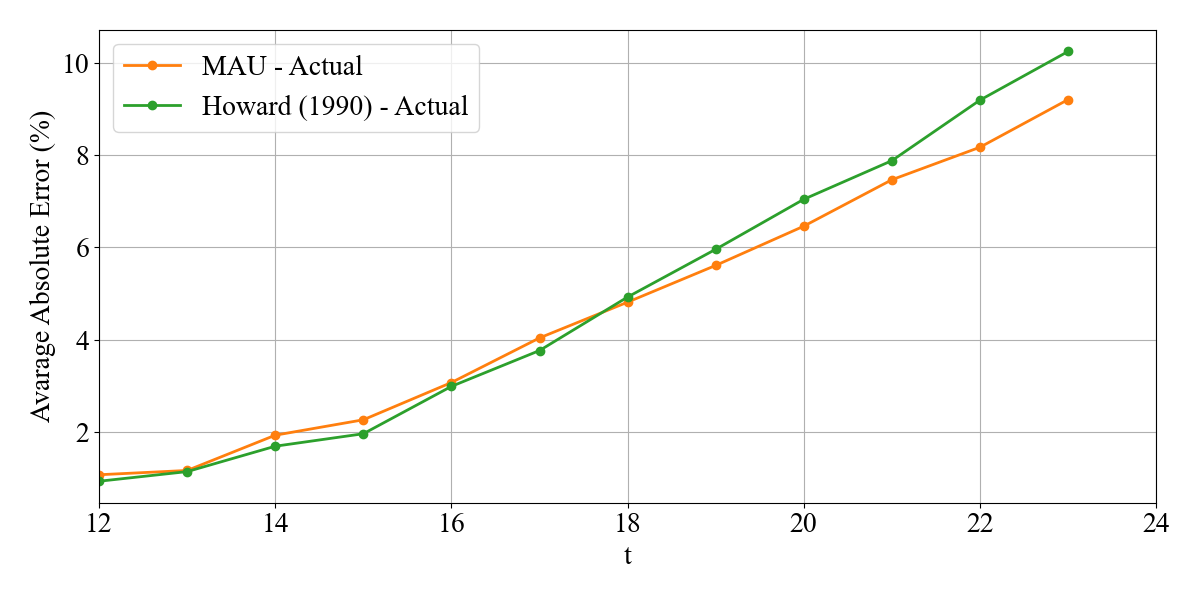
\includegraphics[width=\textwidth]{figures/exp2/error_dr.png}
          \caption{MAUによるテストセットの予測画像と実際の観測画像の平均絶対誤差(オレンジ)と、単純差動回転モデルと実際の観測画像の平均絶対誤差(緑)。}
          \label{fig:exp2_error}
        \end{figure}
        さらに、出力シークエンスの最後のタイムステップにおいて、単純差動回転モデルによるシミュレーションと、実際の観測画像との差異を観察し、動画予測モデルによる出力と比較した。
        このタイムステップは、出力の最後のタイムステップであり、最も不確定性の高い予測である。
        その散布図\ref{fig:exp2_dr_scatter}に示す。
        相関係数は0.97と良好な数値を示しているが、前回実験での同様条件での相関係数は0.98であり、やや低下している。
        また、データ点も若干右下に偏っていることがわかる。
        \begin{figure}[htbp]
          \begin{subfigure}[b]{0.55\textwidth}
            \centering
            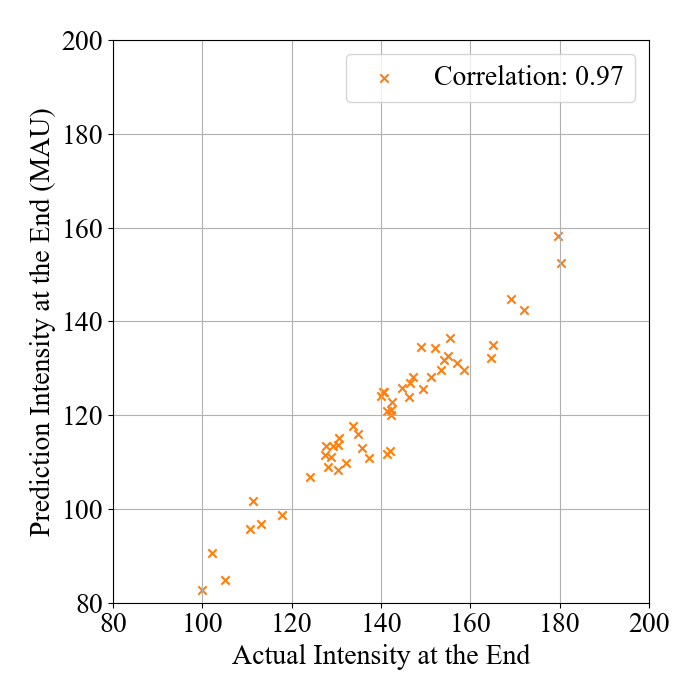
\includegraphics[width=\textwidth]{figures/exp2/intensity_scatter_gt_pd.png}
            \caption{MAUによる、テストセットの最終ステップにおける全球平均輝度の予測対実測の散布図。計算された相関係数は0.97である。}
          \end{subfigure}
          \begin{subfigure}[b]{0.55\textwidth}
            \centering
            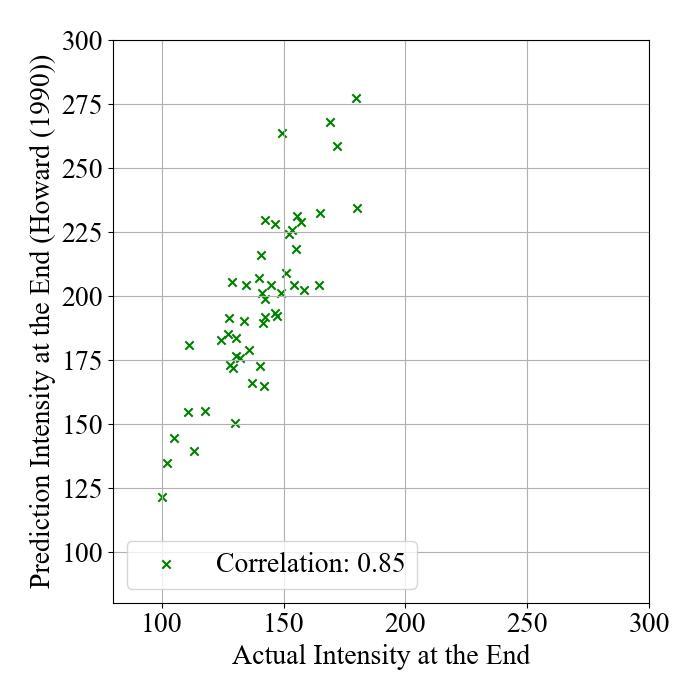
\includegraphics[width=\textwidth]{figures/exp2/intensity_scatter_gt_dr.png}
            \caption{単純差動回転モデルによる、テストセットの最終ステップにおける全球平均輝度の予測対実測の散布図。計算された相関係数は0.85である。}
          \end{subfigure}
          \caption{予測対実測の散布図。縦軸が予測から計算された平均輝度強度、横軸が実際の観測画像から計算された平均輝度強度を表す。}
          \label{fig:exp2_dr_scatter}
        \end{figure}

      \subsubsection{画像類似度}
        前回実験と同様に、画像内での構造的再現度とその時間的変化を評価するために、モデルの出力と対応する時間ステップの実際の観測画像の間のSSIMを計算した。
        SSIMの推移を図\ref{fig:exp2_ssim}に示す。
        画像類似度は、全球での平均輝度と同様に、全球に対してのみ行い、画像中の背景や外縁部からはみ出すコロナなどはその計算に含まれない。
        SSIMの推移の概形は、前回実験の傾向と同様で、ほとんど変化が見られない。
        出力シークエンスの前半では差動回転モデルよりも低い値を示しているが、後半では差動回転モデルよりも高い値を示している。
        \begin{figure}[htbp]
          \centering
          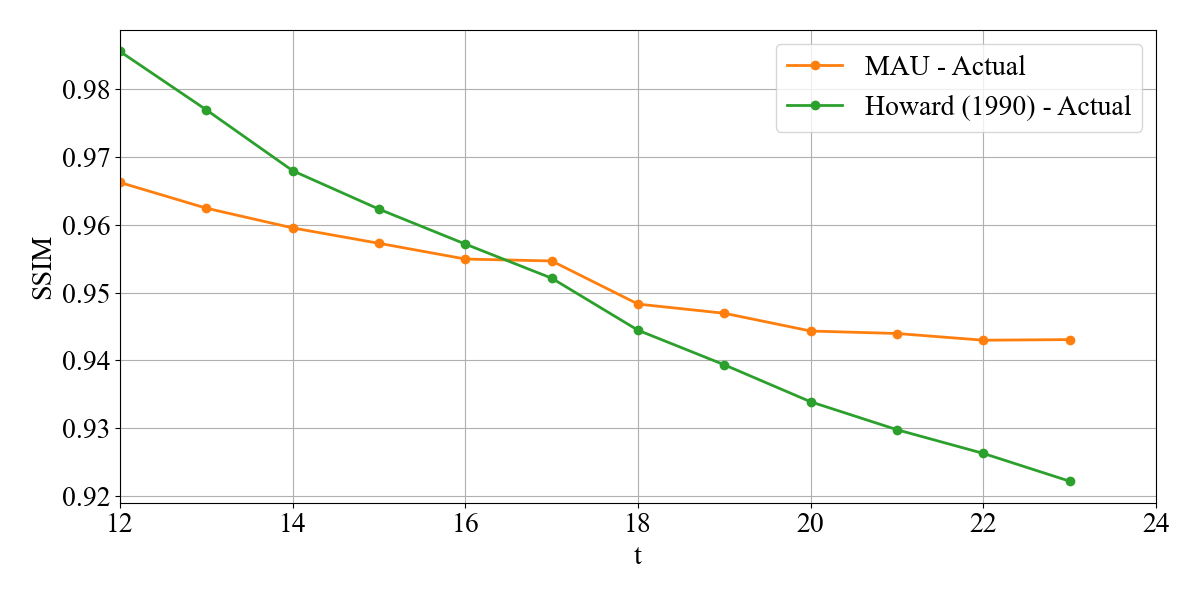
\includegraphics[width=\textwidth]{figures/exp2/average_ssim.png}
          \caption{テストセットでのSSIMの時間推移。SSIMは0から1の値を取り、二つの画像が類似するほど1に近づく。横軸が時間ステップ、縦軸がSSIMを表す。}
          \label{fig:exp2_ssim}
        \end{figure}

% *************************************************************************************************************
        
      \subsection{経度依存性の評価}
        前回実験と同じく、予測性能が経度ごとにばらつきがあるかを確認するために、経度ごと予測の再現度を評価した。分割の方法は前回実験(図\ref{fig:exp1_division_concept})と同様である。
        評価指標には、平均輝度の誤差と、その単純差動回転モデルとの比較を用いた。
        \subsubsection{平均輝度の再現}
          ここでは、全てのテストセットで各セクターごとの平均輝度を計算し、対応する時間ステップの実際の観測画像との絶対誤差を計算した。
            誤差率の時間推移を図\ref{fig:exp2_lng_error}に示す。同時に単純差動回転モデルの経度ごとの画像類似度も計算した。
            経度ごとの誤差率の推移の傾向や時間経過に対する反応は、前回実験とほぼ同様であるが、全体的に数ポイントから10ポイント程度高い値を示している。
            \begin{figure}[htbp]
              \begin{subfigure}{0.5\textwidth}
                \centering
                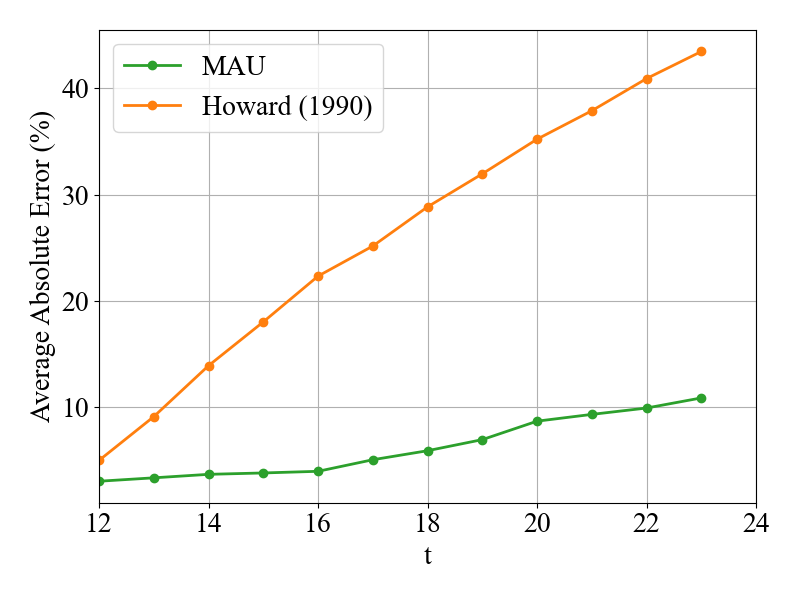
\includegraphics[width=\textwidth]{figures/exp2/lng_error_1.png}
                \caption{-90度から-54度}
              \end{subfigure}%
              \begin{subfigure}{0.5\textwidth}
                \centering
                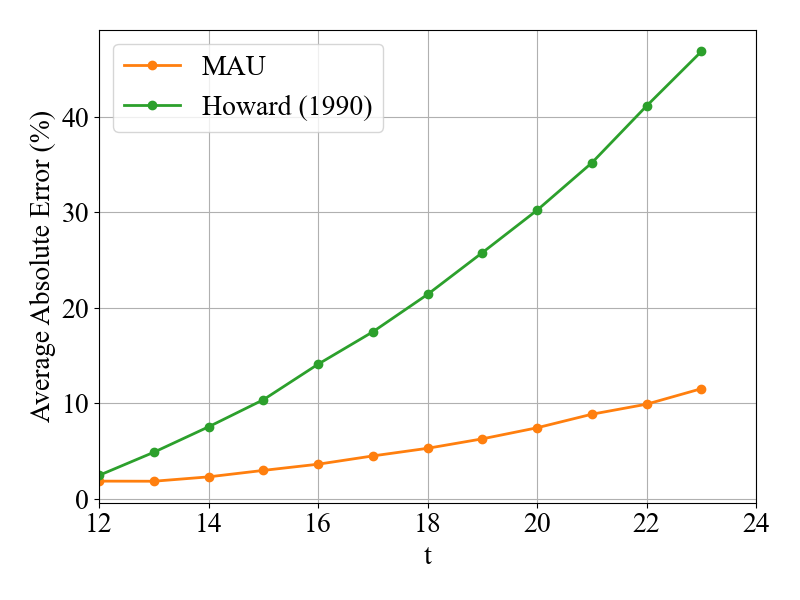
\includegraphics[width=\textwidth]{figures/exp2/lng_error_2.png}
                \caption{-54度から-18度}
              \end{subfigure} \par
              \begin{subfigure}{0.5\textwidth}
                \centering
                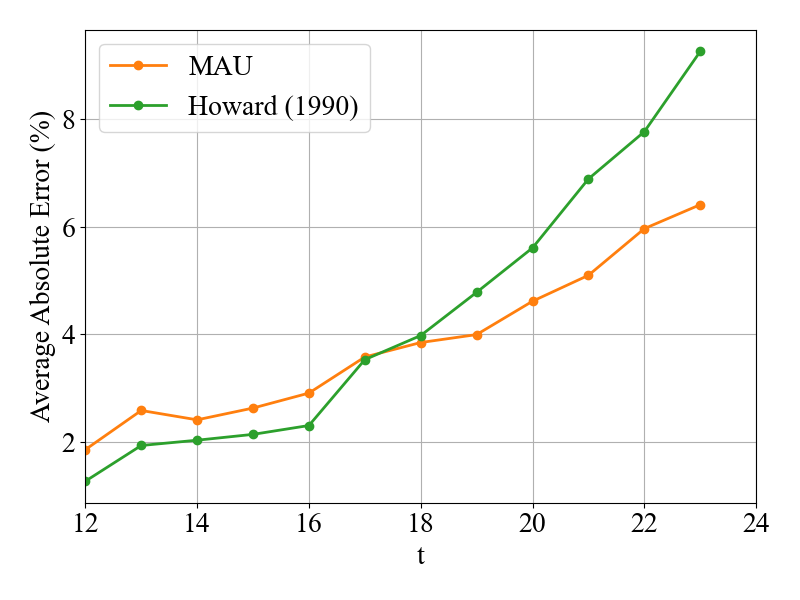
\includegraphics[width=\textwidth]{figures/exp2/lng_error_3.png}
                \caption{-18度から18度}
              \end{subfigure}%
              \begin{subfigure}{0.5\textwidth}
                \centering
                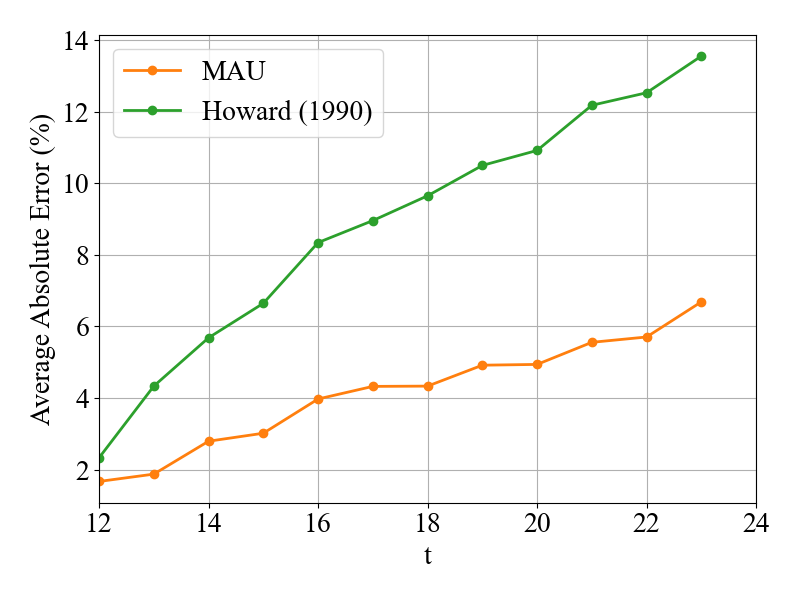
\includegraphics[width=\textwidth]{figures/exp2/lng_error_4.png}
                \caption{18度から54度}
              \end{subfigure} \par
              \begin{subfigure}{0.5\textwidth}
                \centering
                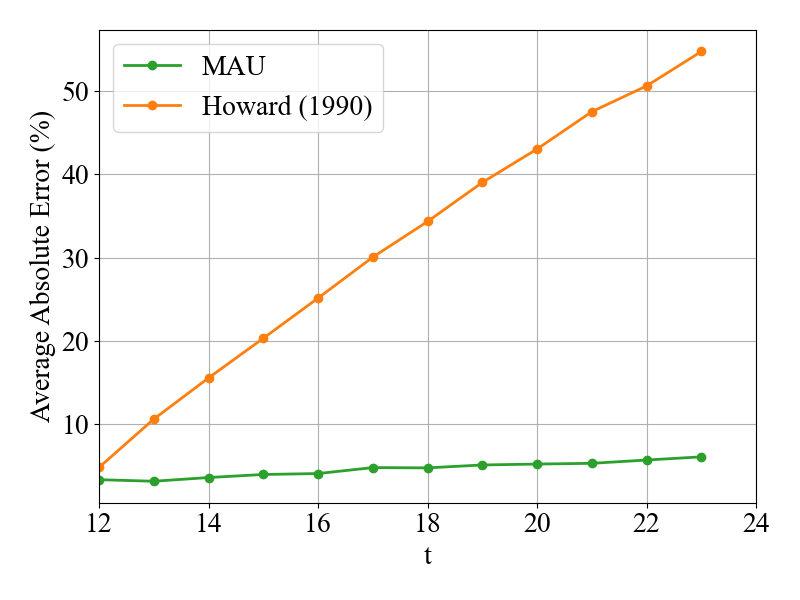
\includegraphics[width=\textwidth]{figures/exp2/lng_error_5.png}
                \caption{54度から90度}
              \end{subfigure}
              \caption{分割された各セクターにおける平均輝度の絶対誤差の時間推移。横軸が時間ステップ、縦軸が平均絶対誤差を表す。各グラフで縦軸の範囲が異なる。緑線がMAUによる予測から計算された絶対誤差、オレンジ線が単純差動回転モデルによるシミュレーションから計算された絶対誤差を表す。}
              \label{fig:exp2_lng_error}
            \end{figure}
          
        \subsubsection{画像類似度}
          全球での場合と同様に、経度ごとにも画像類似度を計算した。その時間推移を図\ref{fig:exp2_lng_ssim}に示す。
          同時に単純差動回転モデルの経度ごとの画像類似度も計算した。
          全球でのSSIMの評価と同様に、経度ごとのSSIMの評価においても、前回実験とほぼ同様の結果となっている。
          \begin{figure}[htbp]
            \begin{subfigure}{0.5\textwidth}
              \centering
              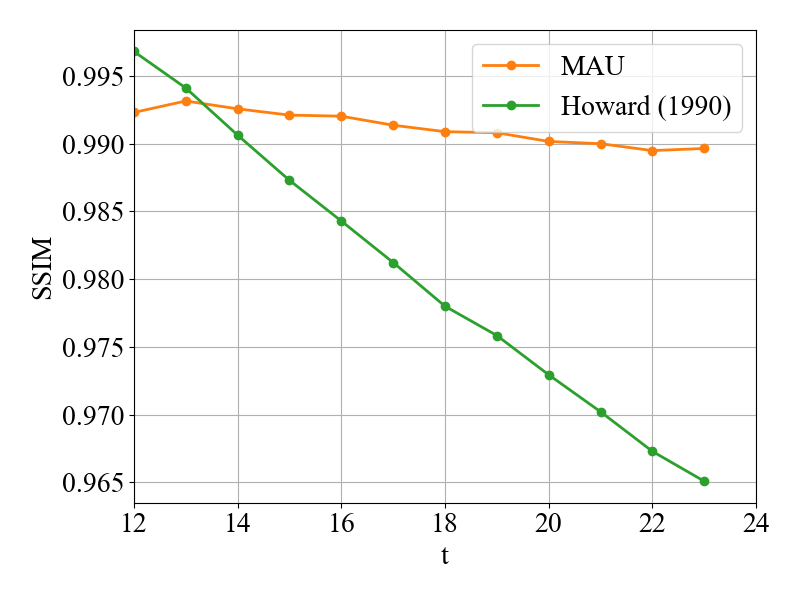
\includegraphics[width=\textwidth]{figures/exp2/lng_ssim_1.png}
              \caption{-90度から-54度}
            \end{subfigure}
            \begin{subfigure}{0.5\textwidth}
              \centering
              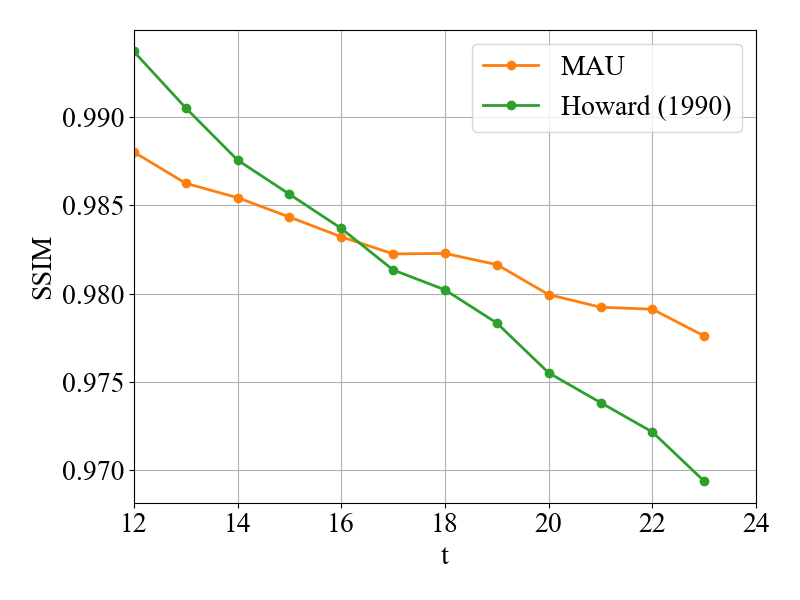
\includegraphics[width=\textwidth]{figures/exp2/lng_ssim_2.png}
              \caption{-54度から-18度}
            \end{subfigure} \par
            \begin{subfigure}{0.5\textwidth}
              \centering
              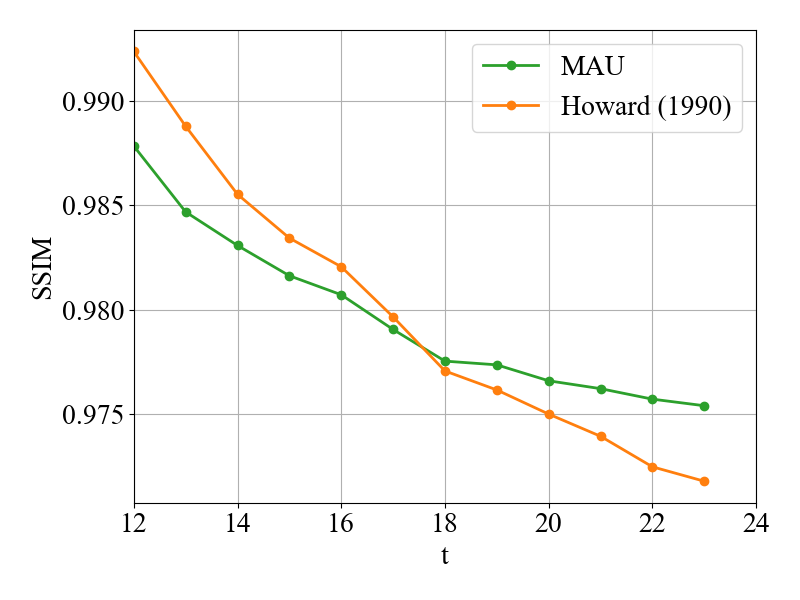
\includegraphics[width=\textwidth]{figures/exp2/lng_ssim_3.png}
              \caption{-18度から18度}
            \end{subfigure}
            \begin{subfigure}{0.5\textwidth}
              \centering
              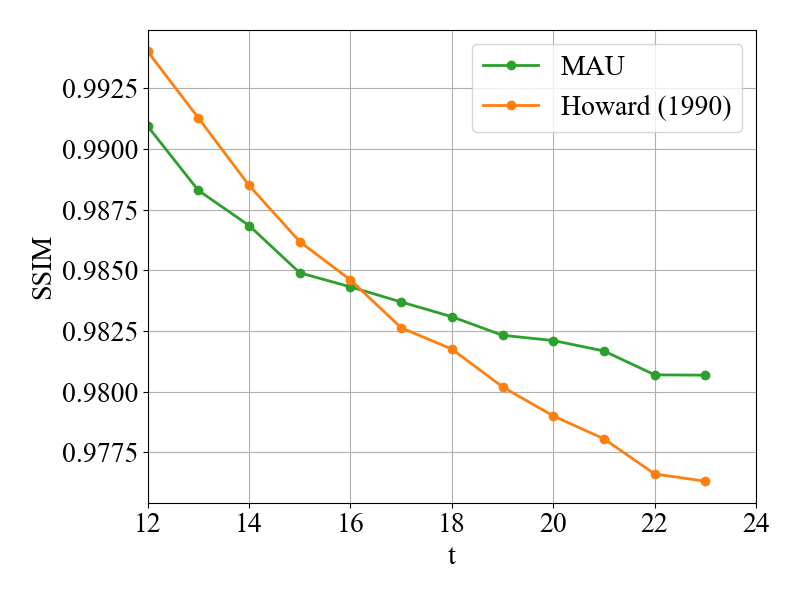
\includegraphics[width=\textwidth]{figures/exp2/lng_ssim_4.png}
              \caption{18度から54度}
            \end{subfigure} \par
            \begin{subfigure}{0.5\textwidth}
              \centering
              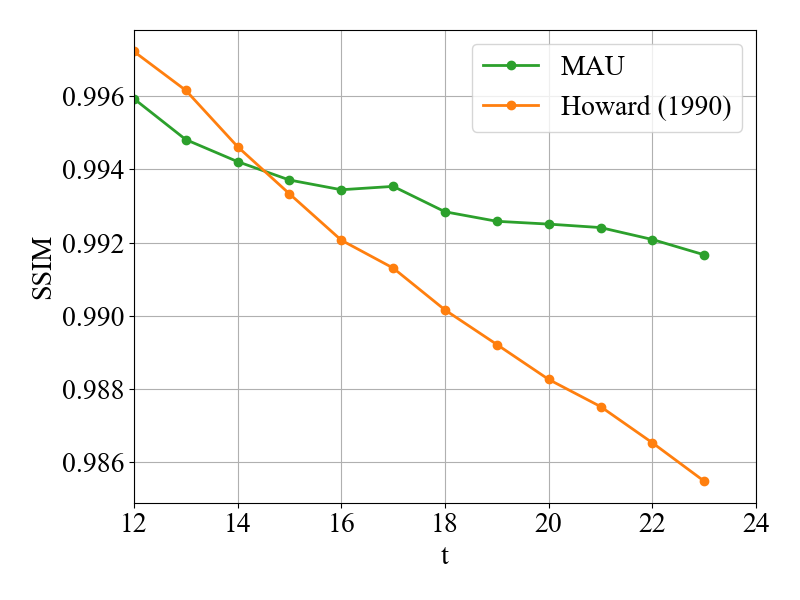
\includegraphics[width=\textwidth]{figures/exp2/lng_ssim_5.png}
              \caption{54度から90度}
            \end{subfigure}
          \caption{分割された各セクターにおけるSSIMの時間推移。横軸が時間ステップ、縦軸がSSIMを表す。各グラフで縦軸の範囲が異なる。緑線がMAUによる予測から計算されたSSIM、オレンジ線が単純差動回転モデルによるシミュレーションから計算されたSSIMを表す。}
          \label{fig:exp2_lng_ssim}
        \end{figure}

% *************************************************************************************************************

    \subsection{東側外縁部に対する評価}
        前回実験と同様に、ここでは東側外縁部に対する評価を行った。
        まず、東側外縁部の平均輝度の再現度を評価した。
      \subsubsection{活動領域に対する視覚的評価}
        ここでは、動画予測モデルが、東側外縁部から出現する活動領域に対して、どのような予測を行っているかを視覚的に評価する。
        前回実験と比較を行うため、同じ期間の同様のデータを示す予測画像を検証する。
        ここで示す画像は、上段が実際の観測画像、下段がその予測画像である。
        出現する活動領域をバウンディングボックスで囲っている。
        図\ref{fig:exp2_limb_example_1}は、活動領域が東側外縁部の北側中緯度帯から出現する例である。
        図\ref{fig:exp2_limb_example_2}は、活動領域が東側外縁部の南側中緯度帯から出現する例である。
        バウンディングボックスを確認すると、前回実験と近い、活動領域の出現箇所への高輝度領域の出現はあることがわかる。
        しかし、前回実験よりもぼやけが激しく、活動領域の形状が顕著に不明瞭になっている。
        \begin{figure}[htbp]
          \centering
          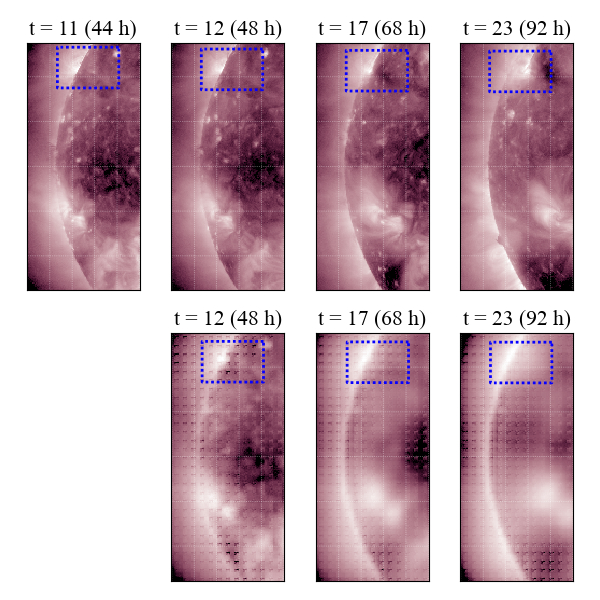
\includegraphics[width=\textwidth]{figures/exp2/limb_sample_3_caption.jpg}
          \caption{東側外縁部の北側中緯度帯から出現する活動領域をもつ予測の例。上段が実際の観測画像、下段がその予測画像である。活動領域を青色破線のバウンディングボックスで囲んでいる。2022年11月6日0時から2022年11月9日8時の期間の画像。}
          \label{fig:exp2_limb_example_1}
        \end{figure}
        \begin{figure}[htbp]
          \centering
          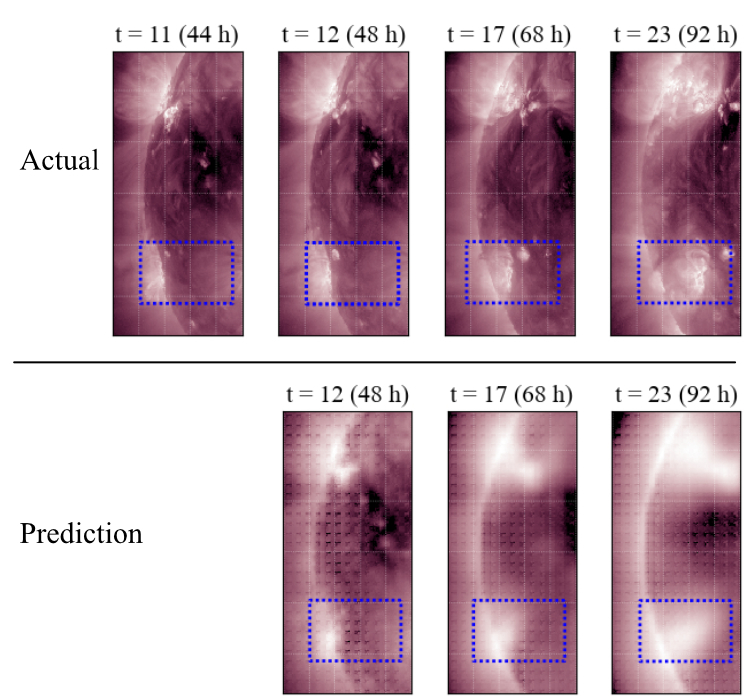
\includegraphics[width=\textwidth]{figures/exp2/limb_sample_12_caption.jpg}
          \caption{東側外縁部の南側中緯度帯から出現する活動領域をもつ予測の例。上段が実際の観測画像、下段がその予測画像である。活動領域を青色破線のバウンディングボックスで囲んでいる。2022年12月12日0時から2022年12月15日8時の期間の画像。}
          \label{fig:exp2_limb_example_2}
        \end{figure}

      \subsubsection{予測対実測散布図による定量的評価}
        さらに、東側外縁部に対する評価を行うために、予測対実測の散布図を作成した。その結果を図\ref{fig:exp2_limb_scatter}に示す。
        相関係数は0.98と、前回同様に高い値を示しているが、1:1の直線からやや外れている。
        \begin{figure}[htbp]
          \centering
          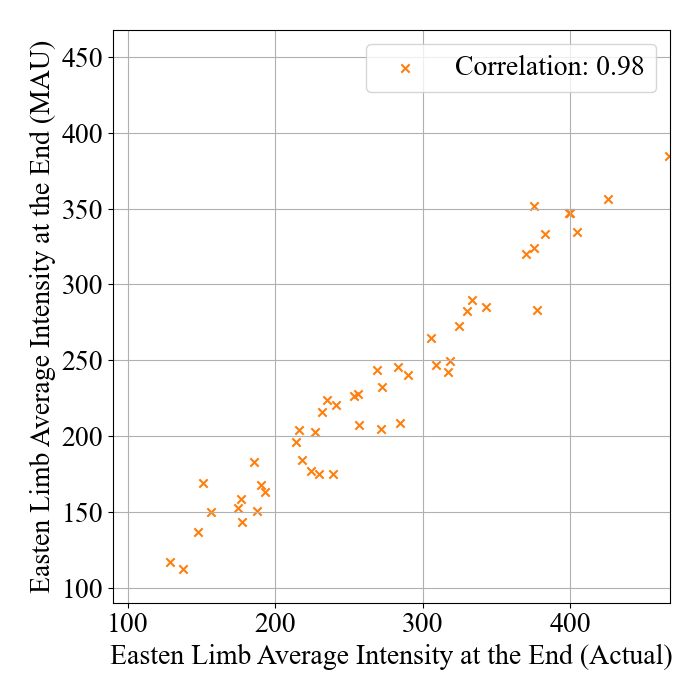
\includegraphics[width=0.5\textwidth]{figures/exp2/limb_scatter_gt_pd.png}
          \caption{すべてのテストセットの、最終タイムステップでの東側外縁部の平均輝度の予測対実測の散布図。横軸が実際の観測画像から計算された平均輝度強度、縦軸がMAUによる予測から計算された平均輝度強度を表す。計算された相関係数は0.98である。}
          \label{fig:exp2_limb_scatter}
        \end{figure}

%%%%%%%%%%%%%%%%%%%%%%%%%%%%%%%%%%%%%%%%%%%%%%%%%%%%%%%%%%%%%%%%%%%%%%%%%%%%%%%%%%%%%%%%%%%%%%%%%%%%%%%%%%%%
        
  \section{考察}
    ここまでの評価結果を表\ref{tab:exp2_result}にまとめる。
    \begin{table}[htbp]
      \centering
      \caption{本実験での各評価の結果。MAUは、本研究で使用した動画予測モデルによる予測に対する評価、\citex{howard1990solar}は、単純差動回転モデルによるシミュレーションに対する評価を表す。すべての数値は、全テストセットの最終タイムステップでの値を平均したものである。}
      \begin{tabular}{lcccccc}
      \hline
      評価指標 & 全球 & \multicolumn{5}{c}{経度ごと} \\
      \cline{3-7}
       &  & -90 to -54 & -54 to -18 & -18 to 18 & 18 to 54 & 54 to 90 \\
      \hline\hline
      平均輝度絶対誤差↓ & & & & & & \\
      \quad MAU - 1波長 & 3.67 & 11.0 & 6.15 & 6.12 & 6.09 & 6.42 \\
      \quad MAU - 3波長 & 9.20 & 17.1 & 11.5 & 6.41 & 6.69 & 14.7 \\
      \quad \citex{howard1990solar} & 10.2 & 81.4 & 46.9 & 9.26 & 13.6 & 35.0 \\
      \hline
      SSIM↑ & & & & & & \\
      \quad MAU - 1波長  & 0.944 & 0.990 & 0.978 & 0.975 & 0.981 & 0.976 \\
      \quad MAU - 3波長 & 0.943 & 0.990 & 0.978 & 0.976 & 0.980 & 0.991 \\
      \quad \citex{howard1990solar} & 0.922 & 0.965 & 0.969 & 0.972 & 0.976 & 0.985 \\
      \hline
      \end{tabular}
      \label{tab:exp2_result}
    \end{table}
    ほとんどの評価指標において、前回実験と比較して、予測性能が低下しているか、ほとんど改善が見られないことがわかる。
    ここでは、その原因を考察する。
    
    \subsection{アーキテクチャと損失関数の問題}
    予測性能の低下の一因として、損失関数の適用性が挙げられる。
    本実験におけるMAUのアーキテクチャでは、3波長のデータを入力としており、出力として用いるのは211Åの波長のみある。
    しかし、モデルにとっての実質的な出力は、171Å、193Å、211Åの3波長のデータである。
    これは、図\ref{fig:exp2_concept}に示すように、出力シークエンスでは、直前のモデルの出力を入力データとして扱うためである。
    これにより、モデルにとっては3波長入力の3波長出力の予測問題となる。
    これはすなわち、損失関数が3波長の全てのチャンネルに対して適用されることを意味する。
    そうなることで、モデルの損失が目的とする211Å以外の波長のデータに影響され、モデルの最適化計算が分散され、結果的に211Åの波長の予測性能が低下している可能性がある。
    
    \subsection{複雑な入力データの相互作用に対するモデルの学習能力の不足}
    前述のような損失関数の構造的問題は、実験設定の段階から可能性として指摘されていた。
    しかし、3波長での場合であっても、それらの相互作用を十分にモデリングできるだけの表現力があれば、この問題は解決でき、さらなる精度向上が期待できると予測されていた。

    そのような背景で行われた本実験であったが、結果として、前回実験と比較して予測性能が低下した。
    これは、3波長という多様な入力データに対して、モデルの表現力が十分でないことを示唆している。
    図\ref{fig:exp2_pd_discuss_1}では、あるテストセットでの、前回実験と本実験での予測画像の拡大画像を示す。
    この予測画像を見ると、全体的なシャープさに欠け、ぼやけた見た目になっていることに加え、画像には特定のノイズパターンが見られる。
    これは、モデルが適切に学習できていないことを示唆している。
    \begin{figure}[htbp]
      \begin{subfigure}{0.5\textwidth}
        \centering
        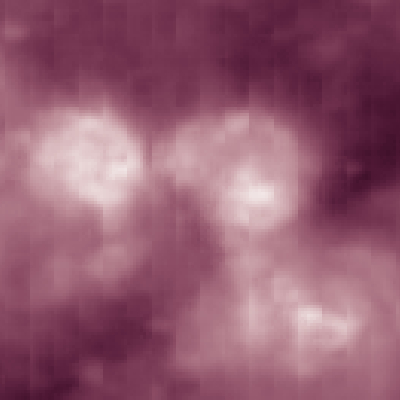
\includegraphics[width=\textwidth]{figures/exp2/sample_exp1.jpg}
        \caption{前回実験}
      \end{subfigure}
      \begin{subfigure}{0.5\textwidth}
        \centering
        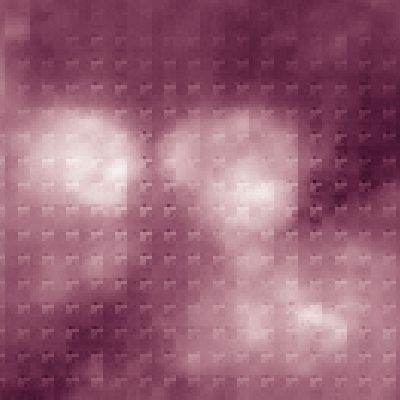
\includegraphics[width=\textwidth]{figures/exp2/sample_exp2.jpg}
        \caption{本実験}
      \end{subfigure}
      \caption{あるテストセットにおける、前回実験(左)と本実験(右)での予測画像の拡大画像。本実験には顕著なノイズパターンが見られる。}
      \label{fig:exp2_pd_discuss_1}
    \end{figure}
    このような現象は、過学習、または学習不足に起因する可能性が高いが、その詳細な原因は不明である。
    しかし、いずれの場合であっても、モデルの表現力が不足していることは明らかである。
    
    \subsection{改善へのアプローチの提案}
      この問題の解決には、以下のようなアプローチが考えられる。
        \paragraph{1波長のみに損失関数を適用するようなアーキテクチャの変更}
          これは、前述の損失関数の問題を解決するためのアプローチである。
          現在のアーキテクチャにおいて、モデルは損失関数を3波長に対して計算している。
          現在のモデルの学習能力では、3波長のデータに対して正確な予測を行うことができない。
          そのため、出力を目的とする1波長に限定し、モデルの学習能力を集中させることで、追加の計算資源を必要とすることなく、より高い予測性能が得られる可能性がある。
          しかし、1波長のみを出力とし、それのみに損失関数を適用する場合、171Å、193Åの波長データには実質的に予測および有効な生成が行われず、それを入力とする出力シークエンス以降での学習が破綻する可能性がある。
          そのため、入力シークエンスでは3波長でのデータを入力とし、出力シークエンスでは1波長のデータのみを入力とするようなアーキテクチャを構成する必要がある。

        \paragraph{より表現力の高いモデルの使用}
          アーキテクチャを変更するアプローチは、損失関数の問題を解決することができるが、3波長のデータに対して正確な予測を行うことができないという問題は解決できない。
          また、出力シークエンスで1波長のみのデータを扱うことで、3波長のデータ間の相互作用を充分に活用できないという問題が生じる可能性がある。
          
          この問題を解決するには、モデルの層を深くするなどの変更を行い、表現力を高めることが考えられる。
          具体的には、空間方向のMAUセルのスタック数を現在の16から32に増やすなどの変更が考えられる。
          これにより、現在よりさらに抽象度の高い情報を詳細に学習したり、より複雑な関係性を学習することができる可能性がある。
          しかし、現在のアーキテクチャの学習には、GPUを用いても30時間程度の時間がかかっている。
          MAUアーキテクチャ全体のパラメータ数のほとんどはMAUセルのパラメータであり、MAUセルのスタック数を増やすことは、学習にかかる時間を線型に増加させる。
          また、モデルの層を深くすることは、モデルの学習難易度を高め、過学習を引き起こす可能性がある。
          それを防ぎ、高い表現力を獲得するためには、さらなる多様的なデータを必要とする可能性があり、下に示すようなデータ増強の必要性が生じる可能性が高い。
          いずれにしても、さらなる高性能なコンピューティング環境や、より長い計算時間が必要となるのは明らかであり、これらの実行には慎重な検討が必要である。

        \paragraph{学習データの増強}
          モデルの学習能力の不足は、データ不足が原因である可能がある。
          前回の実験から、モデルのチャンネルを1から3に増やしたことで、モデルのパラメータ数は3倍になっている。
          当然、入力とするデータの量も、追加波長分で3倍になっているが、それらの相互作用を学習しなければならないという点では、現在よりもっと多くのデータが必要である可能性がある。
          特に、前述のような、さらなるモデルの表現力の向上を目指す場合、より多くのデータが必要となる可能性が高い。
          データの追加には、サンプリング間隔を短縮することで、より多くのデータを取得する方法が考えられる。
          現在は、4時間ごとにデータを取得し、それをそのままモデルの入力としてしている。
          これを、図\ref{fig:exp2_data_sampling_new}のように、新しいサンプリング時刻を追加し、2時間ごとにデータを取得し、二つのシリーズに分割するように変更することが考えられる。
          このようにすることで、モデルにとってのデータ間の時間間隔を変更しないまま、より多様的なデータをモデルに提供することができる。
          \begin{figure}[htbp]
            \centering
            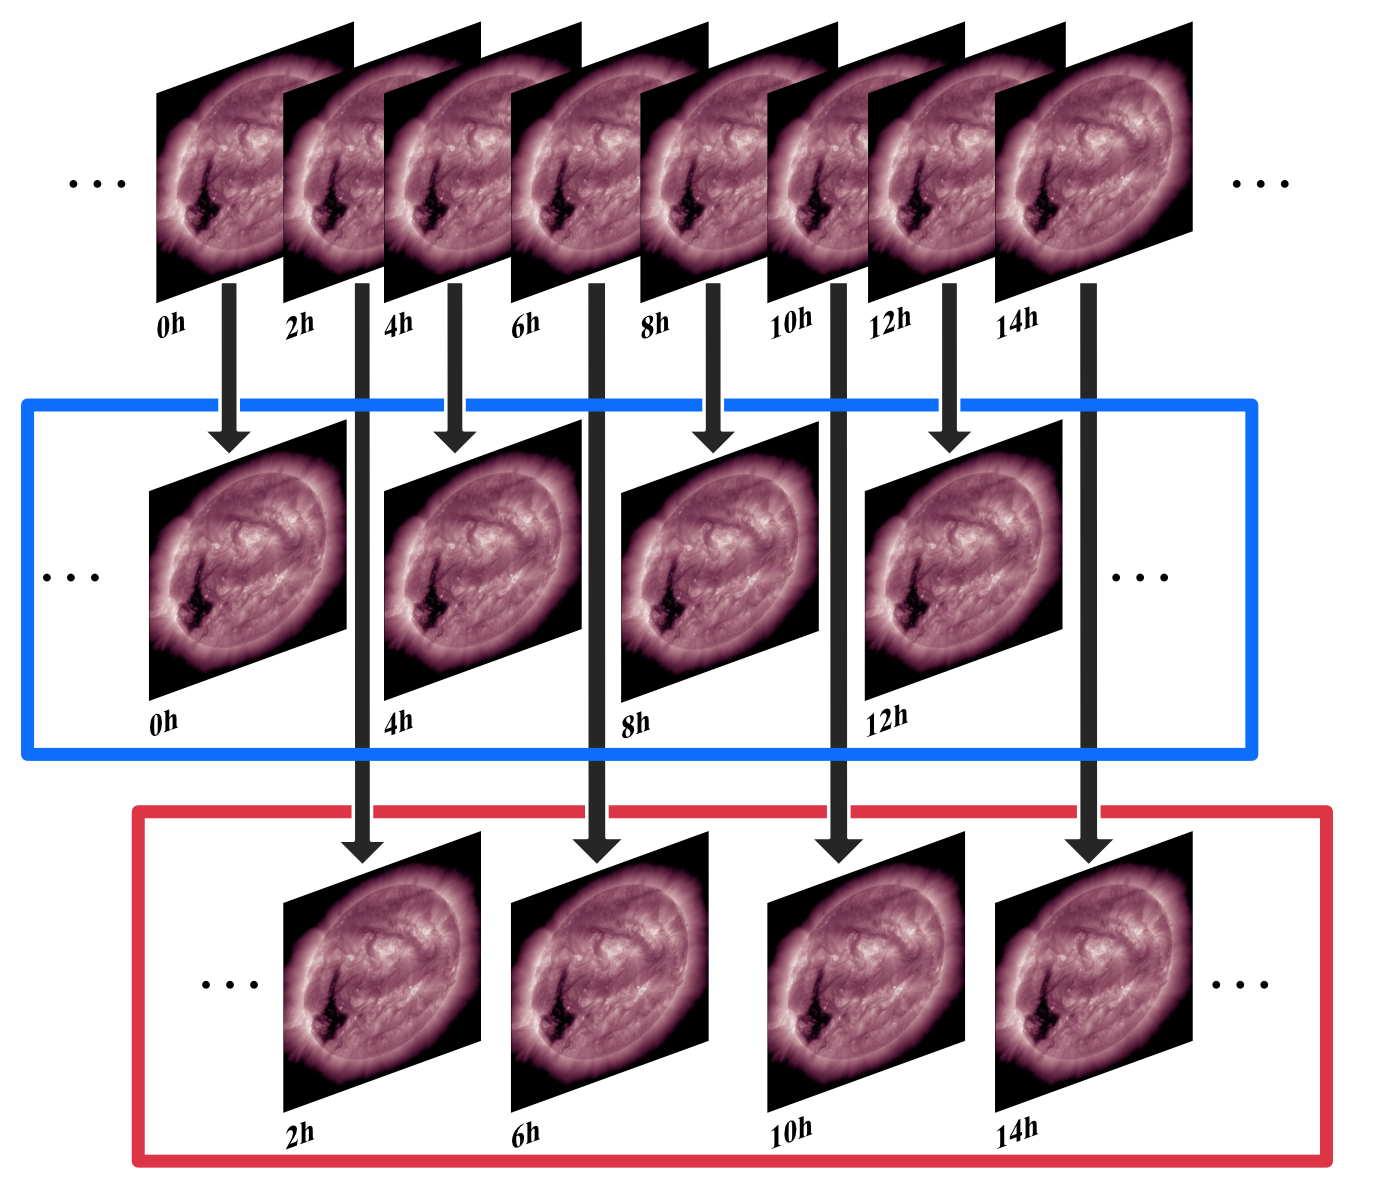
\includegraphics[width=0.9\textwidth]{figures/exp2/exp2_new_dataset.jpg}
            \caption{より高いサンプリング間隔でのデータセット作成方法。短い間隔でサンプリングを行い、それぞれ異なるシリーズ(赤枠、青枠)にすることで、モデルにとっての時間間隔を変えずにデータを増やすことができる。}
            \label{fig:exp2_data_sampling_new}
          \end{figure}
        
    
    % 損失関数の問題
    % 複雑な関係性を捉えられていない
    % 3波長を入力とすることで、モデルの学習が困難になっている
    % ズームした場合の画像の粗さ
    % 画像のぼやけ
    
